\section{Results}
\label{sec:results}

\subsection{No learned method cleared the \texorpdfstring{+10\,pp}{+10 pp} bar against its strongest classical baseline}
\label{sec:k2}

No learned method cleared the bar in any setting. Out of 8 enumerated settings, none has a learned method with a CI above 0 and a gain of at least +10\pp\ (or 10\% RMSE) over the strongest classical baseline (Table~\ref{tab:cross} and Fig.~\ref{fig:forest} give the learned-minus-classical contrast per setting). The positive exceptions compare against weaker baselines: residual PPO against the untuned tracking teacher (+16.7\% RMSE), against the untuned juggling teacher (+292\% median hits; a one-parameter retune also reaches 100 hits), and against the weaker T-adapt of the juggling study (+9.3\pp\ [2.7, 17.3]).

\begin{table*}[t]
\centering
\caption{No learned method beats the strongest classical baseline by the +10\pp\ (or 10\% RMSE) bar in any setting; only the comparison with the weaker R0 does ($^\dagger$). Entries are learned minus strongest classical: success settings in percentage points, tracking in relative RMSE change (positive = learned better). Symbols: R0 is the fitted-parameter classical pipeline on whip (T-adapt3-full), which is no longer the strongest classical there; C-ens is the classical Laplace ensemble with robust plan selection; B is the learned ensemble with robust plan selection; L-est, L-est-full and L-dec4 are learned parameter estimators; T-robust, T-adapt and T-adapt3-full are classical controllers of increasing tooling, C1 and C1-new retuned classical gains; D-canon and D-multi are student training sets from the canonical and the multimodal teacher. S5, S6 PPO rows use the exploration scale chosen by the gate (single seed); the older rows with the default scale are in the source tables. TEST ($n{=}50$) was reused for juggling by three spikes; HOLD was reused (Section~\ref{sec:protocol}). Budget ratios per setting are in Appendix~\ref{app:budget}. The pilot S4 has no row here (see the equivalence summary in Appendix~\ref{app:audit}). This table is generated from result files by \texttt{figures/make\_figs.py}.}
\label{tab:cross}
\small
\begin{tabular}{@{}llrlrl@{}}\toprule
Set. & Learned vs.\ classical & $n$ & Seeds & $\Delta$ [95\% CI] & Learner \\ \midrule
S5 & PPO vs T-robust & 500 & HOLD & $-$23.8 [$-$26.9, $-$20.7] & degrades \\
S6 & PPO vs T-adapt & 500 & HOLD & $-$17.6 [$-$20.3, $-$14.9] & degrades \\
S6 & L-est vs T-adapt & 50 & TEST & $-$15.3 [$-$22.0, $-$8.7] & estimator \\
S7 & PPO vs R0 & 500 & HOLD & $-$2.1 [$-$5.2, +1.1] & not learned \\
S7 & L-est-full vs R0 & 500 & TEST-B & +0.9 [$-$3.5, +5.4] & estimator \\
S7 & L-dec4 vs R0 (H14) & 500 & TEST-C & +6.1 [+1.5, +10.7] & estimator \\
S7 & B vs C-ens (H16a) & 500 & TEST-D & +5.6 [+0.6, +10.6] & estimator + selection \\
S7 & B vs R0 (weaker baseline)$^\dagger$ & 500 & TEST-D & +16.2 [+11.0, +21.4] & estimator + selection \\
S8 & MIP D-canon vs T-adapt3-full & 200 & NEW & $-$12.0 [$-$19.8, $-$4.0] & BC student \\
\midrule
\multicolumn{6}{@{}l}{Tracking, relative RMSE change in \% (positive = learned better)} \\
S1 & PPO vs C1 (W0 clean) & 50 & TEST & $-$7.1 [$-$13.8, +0.3] & RL, 5 seeds \\
S2 & PPO vs C1-new (noise+delay, clean) & 50 & TEST & $-$21.7 [$-$25.7, $-$17.9] & RL, 5 seeds \\
S2 & PPO vs C1-new (noise+delay, disturbed) & 50 & TEST & $-$2.6 [$-$4.5, $-$0.7] & RL, 5 seeds \\
S3 & BC student vs teacher & 500 & HOLD & $-$0.8 [$-$1.0, $-$0.6] & imitation \\
S3 & flow-1 student vs teacher & 500 & HOLD & $-$0.5 [$-$0.7, $-$0.4] & imitation \\
S3 & DDIM-10 student vs teacher & 500 & HOLD & $-$6.2 [$-$6.7, $-$5.7] & imitation \\
\bottomrule\end{tabular}

\end{table*}

\begin{figure*}[t]
\centering
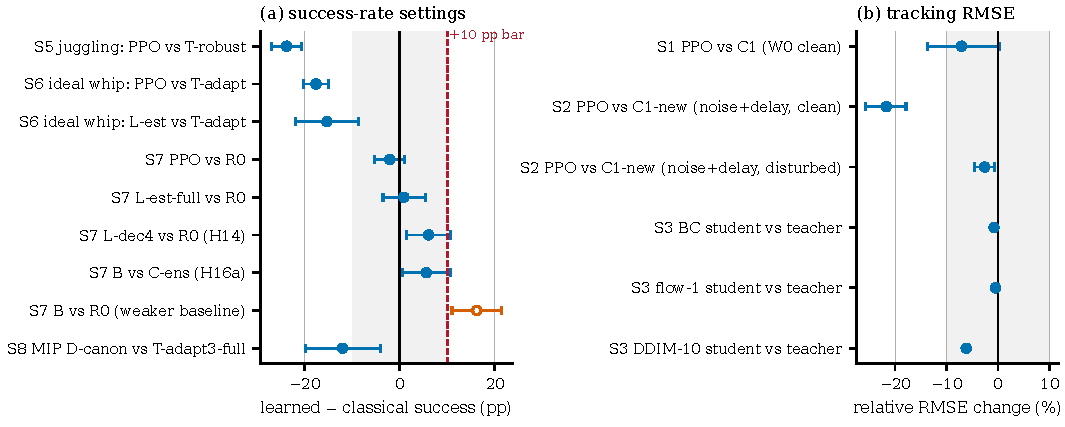
\includegraphics[width=\textwidth]{fig_forest}
\caption{No learned method clears the +10\pp\ bar against its strongest classical baseline; the single hollow point does, but only against the weaker baseline R0 (the fitted-parameter classical pipeline on whip). Learned minus classical across settings. Left: success-rate settings, grey band $\pm10$\pp, dashed line at the +10\pp\ bar. Right: tracking settings in relative RMSE. Bars are 95\% bootstrap CIs; the equivalence (TOST) calls in the text use 90\% CIs, for example [2.2, 9.9] for H14 (L-dec4 vs R0). Evidence sets differ across rows (Table~\ref{tab:cross}).}
\label{fig:forest}
\end{figure*}

Tracking (S1--S3) has little headroom by construction. With a retuned computed-torque controller there is no decisive difference from residual PPO on four clean and disturbed cells (S1: none of the four 90\% CIs decides at $\pm10\%$). With noise and a 30\,ms delay the retuned classical controller is better by 21.7\% clean and 2.6\% disturbed (S2). All five imitation students match the teacher on HOLD with fresh references, 0.5\% to 6.2\% worse in RMSE with CIs inside $\pm10\%$ (S3; the teacher is exact on the clean nominal plant).

In juggling and idealised whip (S5, S6), residual PPO degrades its base. With the gate-chosen exploration scale it loses 23.8\pp\ [20.7, 26.9] and 17.6\pp\ [14.9, 20.3] on HOLD, and 23.0\pp\ and 18.7\pp\ on fresh seeds. The idealised whip base is at 96.8\%, so a +5\pp\ learner effect is impossible there, and for S5 the gate is easy, so it tests plumbing rather than sensitivity.

In realistic whip (S7), neither learned estimators (+0.9\pp\ [$-3.5$, 5.4] on TEST-B) nor PPO ($-2.1$\pp\ [$-5.2$, +1.1]) beat the strongest classical baseline at that time. Eleven PPO and 2 SAC configurations and a 12M-step run all stayed within $-3$ to +2\pp\ of initialisation. Privileged-teacher distillation (S8) leaves all students 12--45\pp\ below T-adapt3-full.

Three of the 8 settings (S5, S6, S7 PPO) had a learner that did not learn, so they cannot show that classical is better. The post hoc TOST rows show equivalence at $\pm10$\pp\ only for some rows (for example S3, S7 estimators and S7 PPO) and clearly worse learners for others; S1 is undecidable and no row has the learner clearly better by more than 10\pp\ (Appendix~\ref{app:audit}). Where we write ``no detectable difference at the +10\pp\ bar'' we do not claim equivalence.

Realistic whip is the setting where headroom is largest, so its history is worth stating in one place. On the locked TEST-B set ($n{=}500$, one evaluation) R0 (T-adapt3-full), the strongest classical baseline at that time, scored 65.6\% [61.4, 69.8], the oracle 89.2\%, and the total headroom was +23.6\pp\ [18.8, 28.4]. The learned estimator with per-link labels (L-est-full) differed from R0 by +0.9\pp\ [$-3.5$, 5.4], and a version without per-link mass labels by $-1.2$\pp\ [$-5.8$, 3.5]; the pre-specified hypothesis that a learned estimator beats R0 by 10\pp\ was not supported. Residual PPO on that set was 0.0\pp\ [$-4.0$, 4.0], but it used the default exploration scale shown by the gate to be unlearnable, so we use the later 3-seed run ($-2.1$\pp) instead. These sets motivated the ladder of Section~\ref{sec:k3}.

Whip is the exception that carries the qualification of K2. Against R0 alone, the learned ensemble B clears the bar on the locked TEST-D set: B$-$R0 is +16.2\pp\ [11.0, 21.4]. But a classical Laplace ensemble, C-ens, also beats R0 by +10.6\pp\ [5.8, 15.4], and against C-ens the learned side is ahead by +5.6\pp\ [0.6, 10.6] (Section~\ref{sec:k3}). C-ens exists because an earlier, unlocked study had shown B ahead of R0; the hypothesis card v9 was written after C-ens was frozen and before TEST-D. A learned advantage of 10\pp\ or more therefore cannot be excluded, and we do not write ``no learned method wins by 10\pp'' without this qualification.

\subsection{On realistic whip, parameters are the largest rung and robust plan selection recovers a large share of that gap}
\label{sec:k3}

On the locked set TEST-C, the true-parameter step is the largest single rung of the headroom ladder. Fig.~\ref{fig:ladder} shows the ladder ($n{=}500$, card v8 committed before the run). The fitted-parameter pipeline R0 reaches 65.6\% [61.4, 69.6]; true parameters (R1) reach 83.2\% [79.8, 86.4]; adding the true chain state (R2) gives 88.6\%; the oracle R4 reaches 93.0\% [90.6, 95.2]. The parameter step R1$-$R0 is +17.6\pp\ [12.6, 22.6] (hypothesis H13 supported, Holm $p=0.00015$). The probe cost R4$-$R2 is +4.4\pp\ [0.8, 7.8]: small but not zero, and the pre-specified bound (upper end below +5\pp) failed (H13b not supported). The chain-state step is R2$-$R1 +5.4\pp\ [1.6, 9.4], and the total headroom R4$-$R0 is +27.4\pp\ [22.6, 32.2]. In the reverse order the chain state first adds +4.8\pp\ [$-0.8$, 10.6] and the parameters then add +18.2\pp\ [13.4, 23.0], so the parameter step is about +18\pp\ in both orders. The same step appeared on the reused HOLD (+16.8\pp\ [12.0, 21.6]) and fresh NEW seeds (+13.0\pp\ [4.5, 21.5]; Appendix~\ref{app:replication}). Parameter estimation is therefore the \emph{largest single rung} of this ladder, not \emph{the} cause: rung sizes depend on order and are not additive.

\begin{figure}[t]
\centering
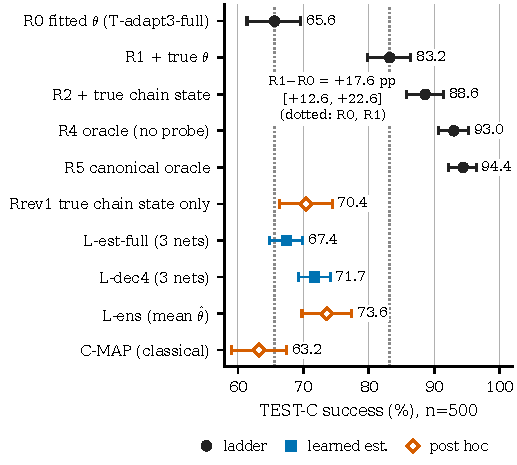
\includegraphics[width=\columnwidth]{fig_ladder}
\caption{Parameter estimation is the largest single rung of the headroom ladder on realistic whip (locked TEST-C), and learned estimators recover only part of it. Rungs: R0 fitted parameters, R1 true parameters, R2 adds the true chain state, R4 oracle planner with no probe time, R5 canonical oracle, Rrev1 true chain state only. Orange open markers are post hoc, descriptive rows. Dotted lines mark R0 and R1. Learned estimators sit between R0 and R1; the classical maximum-a-posteriori (MAP) fit with multi-start sits below R0.}
\label{fig:ladder}
\end{figure}

A learned estimator recovers only part of the parameter gap on TEST-C. The pre-specified estimator duel (H14) compares L-dec4 with R0. L-dec4$-$R0 is +6.1\pp\ with a 90\% CI of [2.2, 9.9], inside $\pm10$\pp, but the Holm-adjusted $p$ is 0.094, so equivalence is \emph{not confirmed} after Holm (the unadjusted TOST passes by 0.1\pp). The estimator recovers 0.34 [0.10, 0.53] of the R0-to-R1 gap, L-est-full 0.10 [$-0.18$, 0.31], and a classical MAP fit with multi-start $-0.14$ [$-0.56$, 0.16] (descriptive). On the reused HOLD the same duel had given +1.1\pp\ [$-3.3$, 5.7], a 4--7\% recovered fraction with a CI that crosses 0; the locked number supersedes it. Parameter error falls a lot (log-damping RMS 0.693 to 0.323) while success moves far less, so precision rather than direction of the error is the issue. Success is also noisy in $\hat\theta$: re-running identical models with float-rounding changes moved HOLD success by up to 3.6\pp.

Robust plan selection recovers a large share of the parameter gap on the locked set TEST-D, for either side. Both selection rules score 8 plus 3 candidate swings (whip plans) in four plausible plants and choose by a worst-case or hit-fraction aggregate. B uses three frozen learned estimators; C-ens uses a Laplace posterior around the classical fit, the same rule on the classical side.

Fig.~\ref{fig:testd} shows TEST-D ($n{=}500$, card v9 committed before the run). R0 reaches 66.4\% [62.2, 70.6], R1 84.4\% [81.2, 87.6] (an R1$-$R0 gap of +18.0\pp), C-ens 77.0\% [73.2, 80.6] and B 82.6\% [79.2, 85.8]. The card's hypothesis H15, that C-ens beats R0, holds: C-ens$-$R0 is +10.6\pp\ [5.8, 15.4]. H15b, that B beats R0, holds: B$-$R0 is +16.2\pp\ [11.0, 21.4]. The share of the R1$-$R0 gap recovered is 0.59 [0.36, 0.82] for C-ens and 0.90 [0.68, 1.16] for B. H16a, that B beats C-ens, holds under Holm: B$-$C-ens is +5.6\pp\ [0.6, 10.6] (Holm $p=0.032$). H16b, that the B advantage is below 10\pp, is \emph{not supported}: the card's rule requires the 95\% CI upper end below +10\pp, and it is 10.6. The card is internally inconsistent here: the rule uses the two-sided 95\% CI, while the Holm step uses a one-sided $p$ that corresponds to the 90\% CI (upper end 9.8, $p=0.043$). We apply the rule text, so a learned advantage of 10\pp\ or more is not excluded.

\begin{figure}[t]
\centering
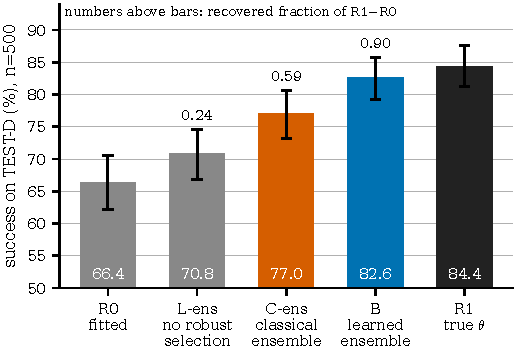
\includegraphics[width=\columnwidth]{fig_testd}
\caption{Robust plan selection recovers a large share of the parameter gap on the locked set TEST-D: 0.59 of the R1$-$R0 gap with the classical ensemble C-ens and 0.90 with the learned ensemble B, which leads C-ens by +5.6\pp. Bars: success with 95\% CI; numbers above the bars: recovered fraction of the R1$-$R0 gap. R0 uses fitted parameters and R1 the true parameters. C-ens is the classical Laplace ensemble with robust plan selection, B the learned ensemble with robust plan selection, and L-ens the same frozen learned estimators as B without robust selection. The y axis starts at 50\%.}
\label{fig:testd}
\end{figure}

A control shows that the gap lies in choosing among candidates rather than in the candidate pool: the best of the executed candidates would have succeeded in 99.8\% of episodes for both runs. The reproduction checks, the agreement of the base candidate with R0 and the winner's-curse effect in the selection of B and C-ens are in Appendix~\ref{app:replication}.

Without robust selection the learned estimators add little on TEST-D. The learned estimator without robust selection gives only +4.4\pp\ [$-1.4$, 10.0] on TEST-D (L-ens, recovered 0.24); on TEST-C the same ensemble gave +8.0\pp\ [2.6, 13.6] (descriptive). The two locked sets differ by several points for the same frozen networks, which fits the noise floor above. Costs differ in the other direction: the classical ensemble needs about 63.3\,s of CPU per episode against 20.4\,s for B, and the learned side paid 13{,}120 training episode-equivalents with simulator labels. Post hoc and descriptive results, not in any verdict, are a 9-network learned ensemble (84.4\% on TEST-D, recovered 1.00 [0.77, 1.29]), the reverse-order ladder, L-ens and C-MAP.

The classical ensemble C-ens recovers 0.59 [0.36, 0.82] of the R1$-$R0 gap without better parameters, and we read this as robust plan selection mattering more than a better point estimate. That reading is an interpretation of the 0.59 fraction, not a test:  averaging the model score over four nearby plants may simply reduce variance in a success rate that is close to chaotic in $\hat\theta$, and we did not test this alternative.

\subsection{A multimodal teacher: canonicalising it helps more than a richer student}
\label{sec:k4}

Canonicalising the teacher helps students more than a richer student does. When the whip teacher is the standard multimodal CMA-ES planner, re-planning the same situation varies by 0.96\,rad RMS, as much as plans for different situations (0.92\,rad); a continuation-warm-started canonical teacher varies by 0.27\,rad within a scenario against 0.73\,rad between scenarios. Replacing the multimodal teacher by the canonical one raised every student's success by 17.5--33.5\pp\ on NEW seeds (BC only, one data size, $n{=}200$; Fig.~\ref{fig:k4} in Appendix~\ref{app:k4}). The best generative student exceeded the MLP by +5.0\pp\ [$-0.3$, 10.2] on the multimodal teacher's data: below the +10\pp\ bar, not an equivalence result, and the best student was identified post hoc. Neither result has locked-set confirmation, and the canonical teacher also changes plan smoothness, so the gain combines multimodality removal with plan regularity.
